% !TeX root = ../main.tex
% Add the above to each chapter to make compiling the PDF easier in some editors.

\chapter{Type Inference}\label{chapter:ti}
The previous chapter discusses the encoding of the type system in Z3. In this chapter, we explain how we build upon this encoding to provide a complete implementation for the static type inference.

\section{Type Inference Design}
We present here the main components of our type inference tool.
\subsection{Abstract Syntax Tree (AST)}
The AST of a program is a data structure which describes the structure of the source code, where each node in the tree represents a construct occurring in the program.

Figure \ref{fig:ast} shows a visualization for the AST of the Python program below.

\begin{lstlisting}
def f():
	return "Hello world!"
f()
\end{lstlisting}
\begin{figure}
	\begin{mdframed}
		\centering
		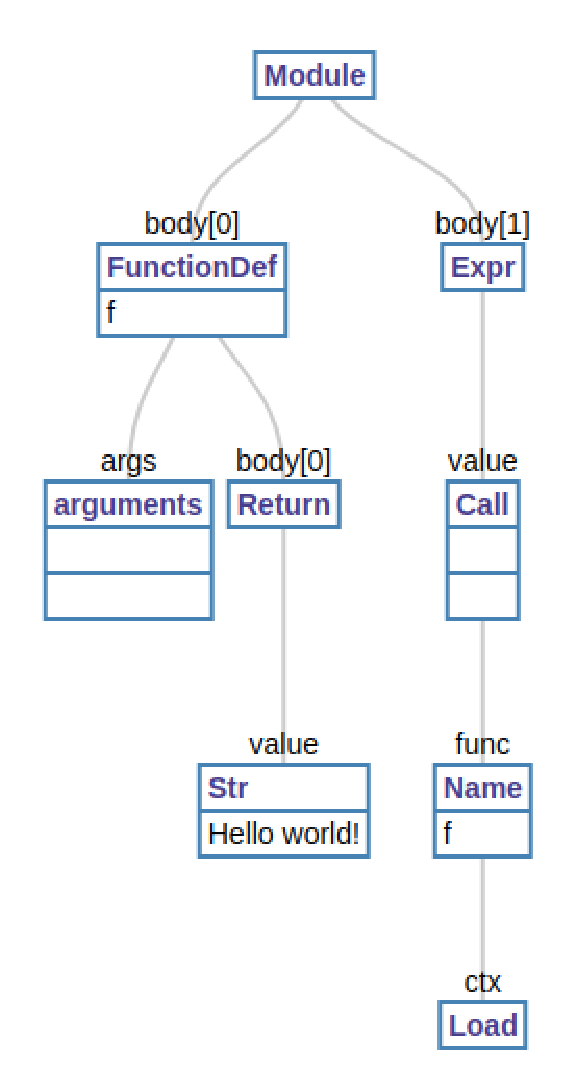
\includegraphics[width=50mm]{images/ast.eps}\\
	\end{mdframed}
	\caption{Abstract Syntax Tree (AST) for a Python program}
	\label{fig:ast}
\end{figure}

Our type inference works by traversing the AST in a depth-first manner, and gathering constraints along the way.
\subsection{Pre-analysis}
Before we attempt to infer the types of the input Python program, some pre-analysis is needed to prepare the configurations of the type inference.

The pre-analyzer takes the AST of the input program and provides the following information:

\begin{itemize}
	\item The maximum length of tuples that appear in the input program.
	\item The maximum length of function arguments that appear in the program.
	\item A mapping from all user-defined classes to their corresponding attributes and methods. It is important to differentiate between two kinds of these attributes: \textit{class-level attributes} and \textit{instance-level attributes}. Class-level attributes are those that are not specific to certain instances, and can be accessed with the class type itself, while instance-level attributes are those which are tied to the class instance during its instantiation or later on. For instance, the class \lstinline|A| in the following example has two attributes, namely \lstinline|x| and \lstinline|y|, where attribute \lstinline|x| is a class-level attribute while \lstinline|y| is an instance-level attribute.
	
	\begin{lstlisting}
class A:
	x = 1
	def __init__(self):
		self.y = 1
		
A.x  # valid
A().x  # valid
A().y  # valid
A.y  # invalid
	\end{lstlisting}
	
	Class-level attributes are detected by the pre-analyzer whenever it encounters an assignment statement in the top-level scope of the class in which the left-hand side is a normal variable.
	
	Instance-level attributes are recognized whenever they are assigned by accessing the first argument in the class methods, like accessing \lstinline|self| argument in the above example.
	
	Note that class-level attributes represent a subset of the instance-level attributes, that is every instance of a certain class can access any class-level attribute. However, instance-level attributes cannot be accessed by the class type itself.
	
	\item A mapping from all user-defined classes to their base classes if they have any.
	\item The inheritance DAG which is used to generate the subtyping constraints discussed in the previous chapter.
\end{itemize}

In addition to the above information, the pre-analyzer also does the following pre-processing to the user-defined classes:
\begin{itemize}
	\item Adds a default \lstinline|__init__| method to classes which do not contain one.
	
	This default \lstinline|__init__| method has the following source:
	\begin{lstlisting}
def __init__(self):
	pass
	\end{lstlisting}
	\item Propagates methods and attributes from base classes to their subclasses. The method resolution order which governs the order of this propagation is discussed later in this chapter.
\end{itemize}

\subsection{Context Hierarchy}
A context contains the information that a certain scope in the program holds. It contains a mapping from the variable names in this context to the Z3 variables representing their types, which are evaluated to the correct types after solving the SMT problem. Every context also has references to its children contexts (which are created inside the scope of this context) and a reference to its parent context.

Below is a listing of the constructs which create new contexts:

\begin{itemize}
	\item \lstinline|if| statements.
	\item \lstinline|for| and \lstinline|while| loops.
	\item Function definitions
	\item Class definitions
	\item List, set and dictionary comprehensions
\end{itemize}

Figure \ref{fig:contexts} shows a tree representing the context hierarchy for the Python program below.

\begin{figure}[H]
	\begin{mdframed}
		\Tree[.{global} [.{A} {f} {g} ] [.{for} {if} {else} ] {list comp} ]
	\end{mdframed}
	\caption{Context hierarchy for a Python program}
	\label{fig:contexts}
\end{figure}

\begin{lstlisting}
x = [1, 2, 3]

class A:
	def f(self):
		pass
	def g(self):
		pass
	
for i in x:
	if True:
		pass
	else:
		pass
		
y = [i + 1 for i in x]
\end{lstlisting}
\subsection{Z3 Solver}
The Z3 solver is the main component in the type inference design. It is responsible for solving all the constraints imposed by the Python program semantics, or report that they are impossible to be satisfied.

We extend the default solver in Z3, such that during the instantiation of every solver instance, the following takes place:

\begin{itemize}
	\item The pre-analysis defined above in processed.
	\item The \textit{type sort} data-type is declared with all its constructors.
	\item The subtyping rules discussed in chapter \ref{chapter:background} are initialized. 
\end{itemize}

At the end of the program inference, this solver is queried for a solution to all the added constraints.

\subsection{Import Handler}
As the name suggests, the import handler is responsible for handling module importing during the type inference.

If the imported module is a built-in Python package, it retrieves the module from the corresponding stub file and infers the types of its contents, otherwise, it reads the imported module from the disk and infers its types in a separate context.\\

We will discuss later in this chapter different types of import statements in Python and how they are handled in our type inference.
\subsection{Stubs Handler}
As discussed earlier, \textbf{stubs} are files containing code which simulates built-in functionalities. A \textbf{stub function} is a function declaration which mocks some other function. The following function is a stub function which mocks the built-in function \lstinline|len|:

\begin{lstlisting}
def len(_: object) -> int:
	...
\end{lstlisting}

Stubs enable the type inference to infer the types of programs which use built-ins. The stubs handler is the module responsible for organizing the relevant stub files which are required by the program being inferred.

\subsection{Annotations Resolver}
PEP 3107 \cite{3107} introduced the ability to add function type annotations, while PEP 484 \cite{484} introduced the semantics for writing such annotations. The annotation resolver is responsible for translating a type annotation encountered in the program into the corresponding type-sort constructor.

For example, the type annotation \lstinline|List[int]| is translated to \lstinline|type_sort.list(type_sort.int)|.\\

We will explain how these type annotations are useful in the type inference when we get to the inference of function definitions.
\subsection{Inference Configuration}
The user of the type inference has the ability to control the behavior of the type inference according to some pre-defined configurations. Each configuration is expected to have its gain and limitation. Some configurations, for instance, lead to a significant increase in the inference speed, yet at the cost of rejecting a larger set of correct programs. We will discuss the current possible configurations when we get to the rules related to these configurations.
\subsection{Hard Constraints vs. Soft Constraints}
An important addition to our type inference was introducing the ability to add soft constraints. \textbf{Hard constraints} are the constraints that \textbf{must} be satisfied by the program, such that if at least one hard constraint cannot be satisfied, the program is rejected and cannot type. On the other hand, \textbf{soft constraints} are those that are good to be satisfied, but they are not obligatory, such that a program violating some soft constraints is not rejected by the type inference. See the following example for illustration:

\begin{lstlisting}
def f(x):
	y = [1, 2, 3]
	return y[x]
\end{lstlisting}

Here, the array \lstinline|y| is indexed with variable \lstinline|x|. Therefore, the type of \lstinline|x| \textbf{must} be a subtype of \lstinline|int|, so a program in which the type of \lstinline|x| violates this constraint (e.g., having \lstinline|x| as a float) would be rejected. The constraint in this case is a hard one. Another hard constraint is added in the assignment statement \lstinline|y = [1, 2, 3]|, that the type of the array literal \lstinline|[1, 2, 3]| is a subtype of the type of variable \lstinline|y|. Moreover, a soft constraint is added that both the type of the array literal and the type of \lstinline|y| are the same. Without this soft constraint, the type of \lstinline|y| in the model given by Z3 might be an \lstinline|object|, or any super type of the right-hand side (which is correct and sound, but not very accurate). So the purpose of the hard constraints is to provide a sound type inference, while that of the soft constraints is to increase its accuracy.
\section{Type Inference Rules}
Having explained the main components of the type inference, we are now ready to discuss the axioms added for every construct in the Python program.
\subsection{Expressions Rules}
An \textit{expression} is any language construct that evaluates to a value. It can be a combination of one or more values, variables, operators and function calls. Every construct in Python that can be printed is an expression.

Below are some examples of Python expressions:
\begin{lstlisting}
1 + 2 / 3
-a
[1.2, 2.0, b]
[[1.1, 2.5], c]
{(i, i * 2) for j in d for i in j}
2 & 3
d[f]
(g, 2.0, a)
"string"
(1 is 2) + 1
i[o]
\end{lstlisting}

We present here the axioms that are generated by every expression in Python.

\subsubsection{List and Set Literals}
As discussed earlier, the elements of a single list or a set have to be homogeneous, that is all these elements have to be of the same type.

So the elements type of a list (or a set) literal is the super type of all the list element.

Assuming a function \lstinline|infer| which takes the AST node of the expression and returns its inferred type, the inference of list literals is implemented as follows:

\begin{lstlisting}
def infer(node):
	...
	if isinstance(node, ast.List):
		elements = node.elts
		elements_type = new_z3_constant()
		
		for element in elements:
			current_element_type = infer(element)
			add_axiom(subtype(current_element_type, elements_type))
			
		return type_sort.list(elements_type)
	...
\end{lstlisting}

For example, the type of the list literal \lstinline|[1, 2.0, 3j]| is \lstinline|List[complex]|, since we assume \lstinline|complex| to be a super type of \lstinline|int| and \lstinline|float|.\\

The inference for sets is exactly the same after replacing the list z3 constructor with the set one.


\subsubsection{Dictionary Literals}
Similar to lists and sets, dictionaries should have homogeneous keys set and values set, and the type inferred for each of these sets is the super type of its elements. For example, the type inferred for the dictionary \lstinline|{1: "string", 2: 3.6}| is \lstinline|Dict[int, object]|, because \lstinline|object| is the common super type between \lstinline|str| and \lstinline|float|.


\subsubsection{Tuple Literals}
The type of the tuple includes information about the types of all its elements. So to get the type of the tuple, we first infer the types of all its elements. For example, the type of the tuple \lstinline|(1, "string", object())| is \lstinline|Tuple[int, str, object]|

\subsubsection{Binary Operations}
Binary operations are the operations which combine two expressions, called operands, to produce a result expression. The inference of binary operations in Python is not very straightforward because the result type from every operation depends on different combinations of the types of the operands. We discuss here the axioms generated for every binary operation supported by Python.\\

\textbf{Addition (+)}
The addition operation is either a numeric addition or a sequence concatenation. For the numeric addition, the type of the result is the super type of the types of the operands. This is encoded in Z3Py as follows:

\begin{lstlisting}
Or(
	And(subtype(left, type_sort.complex), subtype(right, left), result == left),
	And(subtype(right, type_sort.complex), subtype(left, right), result == right)
)
\end{lstlisting}

As for sequence concatenation, there are different cases to consider:

\begin{itemize}
	\item Lists concatenation: The result type is a list in which the type of the elements is a super type of elements in both operands.
	\item String (or byte string) concatenation: The two operands should be of the same type.
	\item Tuple concatenation: The resulting type should be a tuple with the elements types of both operands concatenated.
\end{itemize}

For simplicity, we do not write the axioms for the sequence concatenation here.

Also, we do not currently consider operator overloading. However, this is not rejected by principle, these axioms can be extended to include classes which contain the method \lstinline|__add__|.

The listing below shows examples for the addition operation and their inferred types:

\begin{lstlisting}
1 + 1.0  # float
1j + 1.0  # complex
[1, 2, 3] + [4.0, 2]  # List[float]
"a" + "b"  # str
(1, "st") + (2.0, object())  # Tuple[int, str, float, object]
[1, 2, 3] + "a"  # Invalid
\end{lstlisting}

\textbf{Multiplication (*)}
Multiplication in Python, also without considering operator overloading, is either numeric multiplication or sequence repetition.

Similar to addition, the result type of numeric multiplication is the super type of the types of the operands. In case of sequence repetition, one of the operands must be a subtype of \lstinline|int| and the other one should be the sequence. In all the sequences except tuples, the result type is the same as the sequence being multiplied. Ideally in case of tuples, the result is a tuple type with the argument types of the operand tuple repeated by the operand number. However, resolving the exact numeric value is impossible statically. Therefore, we consider the result of tuple multiplication to be the same type as the operand tuple. This is sound because no new types are introduced in the tuple arguments after multiplication, and as we will see shortly, any operation on tuple (e.g., indexing) does not care about the order of the types of the tuple elements. So the two tuple types \lstinline|Tuple[int, str]| and \lstinline|Tuple[int, str, int, str]| give the same output after applying any operation on the tuple.\\

An important thing to notice in both addition and multiplication is that applying these operations on two \lstinline|bool| types results in an \lstinline|int| type. So this needs special handling during the axioms generation..

\begin{lstlisting}
3 * 4.0  # float
[1, 2, 3] * 3  # List[int]
(1, 2) * 2  # Tuple[int, int]
True * False  # int
[1, 2] * 3.0  # invalid
\end{lstlisting}

\textbf{Division (/)} Division is only applicable on numeric types. The result is \lstinline|complex| if at least one of the operands is of \lstinline|complex| type, otherwise it is a float. Note that this is different from floor division (//).

The axioms generated by a division operation are given below:

\begin{lstlisting}
And(
	types.subtype(left, type_sort.complex), types.subtype(right, type_sort.complex),
	Implies(Or(left == type_sort.complex, right == type_sort.complex), result == type_sort.complex),
	Implies(Not(Or(left == type_sort.complex, right == type_sort.complex)), result == types.float)
)
\end{lstlisting}

\textbf{Other Arithmetic Operations (-, //, **, \%)}
The remaining arithmetic operations (subtraction, floor division, exponentiation, modulo operator) exhibit similar behavior in terms of type inference. They can only be applied on numeric types and the result type is the super type of the types of the operands. \\

There is a single special case to consider in the modulo operator (\%). In addition to giving the division remainder, it can also be used in string formating. Therefore, a disjunction is added to the axioms in this case that the left operand is a \lstinline|str| type without restricting the right operand.

\begin{lstlisting}
"A string which contains a number %i}" % 1
\end{lstlisting}

\textbf{Bitwise Binary Operations (\&, \textrm{\^}, |, <<, >>)}
Bitwise operations can only be applied on subtypes of \lstinline|int| types (\lstinline|int| and \lstinline|bool|). The result is \lstinline|int| in all cases except when we apply \&, \textrm{\^} or | on two \lstinline|bool| types, where in such case the result is \lstinline|bool|.

\subsubsection{Unary Operations}
Unary operations are the operations which are only applied on only one expression, called operand and gives a result expression. The supported unary operations in Python are unary \lstinline|-| (minus), unary \lstinline|+| (plus), unary \lstinline|~| invert, and \lstinline|not|.\\

For the plus and minus unary operations, the operand must be a subtype of \lstinline|complex|, and the result is \lstinline|int| if the type of the operand is \lstinline|bool|, otherwise it is the same type as the operand. As for the unary invert, the operand must be a subtype of \lstinline|int|, and the result is always of type \lstinline|int|.

The \lstinline|not| operation can by applied on any object and result in a \lstinline|bool| type.


\subsubsection{Boolean Operations}
There are two boolean operators in Python: \lstinline|and| and \lstinline|or|.

Before explaining the inference for these operations, it is important to understand what a \textit{truth value} of an object is.

In Python, every object can be tested for truth value, where each object can evaluate to \lstinline|True| or \lstinline|False| when used as test condition in \lstinline|if| or \lstinline|while| statements or in a boolean operation. The following values have a \lstinline|False| truth value:
\begin{itemize}
	\item \lstinline|None|
	\item \lstinline|False|
	\item Zero numeric value: 0, 0.0, 0j
	\item Any object which has \lstinline|__len__| method which returns a zero.
\end{itemize}
Any other object has a \lstinline|True| truth value. \\

The result type from a boolean operation is not simple to infer, since it totally depends on the values that the operands carry during runtime, and these values are impossible to be statically resolved. Specifically, the \lstinline|and| operator keeps evaluating the operands until an operand with a \lstinline|False| truth value is encountered. \lstinline|or| operator does the opposite. See the following example for illustration:
\begin{lstlisting}
a = function_which_returns_int()
b = function_which_returns_string()

x = a and b
y = a or b
\end{lstlisting}

If \lstinline|a| has a zero value during runtime, then the type of \lstinline|x| will be the same as \lstinline|a|, which is \lstinline|int|, otherwise it will be \lstinline|str|. Conversely, \lstinline|y| will have type \lstinline|str| if \lstinline|a| has a zero value, otherwise it will have an \lstinline|int| type.

As mentioned, the values of \lstinline|a| and \lstinline|b| are impossible to be statically resolved. Therefore, the type of the result from a boolean operation is inferred to be the common super type between its operands.

So the result from \lstinline|1 and 2.0| is \lstinline|float| and from \lstinline|1 and "str"| is \lstinline|object|.

\subsubsection{If (Conditional) Expression}
With an if expression, conditional statements can be written as one statement which returns a value depending on whether a certain condition is true or false.
\begin{lstlisting}
x = A if some_condition else B
\end{lstlisting}
This does the exact same thing as the following:
\begin{lstlisting}
if some_condition:
	x = A
else:
	x = B
\end{lstlisting}

The inferred type for the if expression value is the common super type of the types of the true (A) and the false (B) values.

\subsubsection{Subscripts}
Subscript literals in Python are any literals which end in square brackets containing some expression. For example, all the following are subscript literals:
\begin{lstlisting}
x[a]
x[a:b]
x[f()]
\end{lstlisting}

There are two kinds of subscripts in Python: \textit{indexed} subscript and \textit{sliced} subscript. A sliced subscript is that which contains one or two colons \lstinline|:|. Any other subscript is an indexed subscript. \\

In python, any type which contains \lstinline|__getitem__| method can be indexed or sliced. However for simplicity, we only consider built-in types here. We explain later in this chapter how we enhance the type inference to account for user-defined classes which implement the \lstinline|__getitem__| method. \\

In our type system, only strings (and byte strings), lists, dictionaries and tuples support \textbf{indexing}:

\begin{itemize}
	\item For strings, the index must be a subtype of \lstinline|int| and the result is a \lstinline|str|.
	\item For lists, the index is a subtype of \lstinline|int| and the result is the type of the list elements.
	\item For tuples, the index must be a subtype of \lstinline|int|, and the result is the common super type between all the tuple elements. This is because it is not possible to statically resolve the value of the index, so we cannot know which element the indexing is referring to. For this reason, the order (or the repetition) of the types of the tuple elements does not matter in indexing. For example, indexing both tuples of types \lstinline|Tuple[int, float]| and \lstinline|Tuple[int, float, int]| will give the same result type, \lstinline|float|.
	\item For dictionaries, the index type should be the same as the inferred type of the dictionary keys, and the result type is the type of the dictionary values.
\end{itemize}

As for \textbf{sliced} subscripts, only strings, lists and tuples support slicing. The slicing one or more keys must be a subtype of \lstinline|int|. The result type from slicing is the same as the sliced object. For the same reason stated above, slicing the tuple results in the same tuple type because resolving the slicing ends is impossible statically. This is also sound because any operation applied on the result from slicing a tuple should be compatible with every element type in the original tuple.

\subsubsection{Comprehensions}
Comprehensions are constructs which enable the programmer to create lists, sets or dictionaries in a natural and elegant way from any other iterable object.

The following set comprehension creates a set \lstinline|x| which contains the square of all values in another iterable \lstinline|y|.

\begin{lstlisting}
x = {i * i for i in y}
\end{lstlisting}

This is equivalent to the following in a mathematical syntax:
\begin{lstlisting}[language=, mathescape]
x = {i * i | i $\in$ y}
\end{lstlisting}

The expression \lstinline|i in y| in the above example is called a \textit{generator expression} while the expression \lstinline|i * i| is called the comprehension element.

The inference for comprehensions works by creating a local context for the generator, and inferring the generator target (\lstinline|i| in the example above) in this local context according to the generator iterable (\lstinline|y|). Then by having the target inferred in the local context, the type of the comprehension element can be inferred by applying the expressions inference rules on it.

For the example above, assuming the type of \lstinline|y| is inferred to be \lstinline|List[int]|, then the type of \lstinline|i| is inferred as \lstinline|int| in the local context of the generator expression. Then the type of the set elements is inferred from the multiplication inference rules explained above: \lstinline|int * int := int|. So the comprehension result will have a result of \lstinline|Set[int]|. \\

Moreover, the generator expressions can be chained (nested). See the following example for illustration:

\begin{lstlisting}
x = [[1, 2, 3],
     [4, 5, 6],
     [7, 8, 9]]
	 
y = [i for j in x for i in j]
\end{lstlisting}

The array \lstinline|y| contains the array \lstinline|x| after flattening all its inner arrays (\lstinline|[1, 2, 3, 4, 5, 6, 7, 8, 9]|). The inference for chained generators works by inferring the generator targets in the order they appear in the comprehension. So the type of \lstinline|j| in the above example is inferred to be \lstinline|List[int]| (because \lstinline|x| is \lstinline|List[List[int]]|), and the type of the second generator target \lstinline|i| (which is also the comprehension element) is inferred to be \lstinline|int|, and the type of y is then \lstinline|List[int]|.

In addition to generators chaining, the comprehension itself can be nested.
\begin{lstlisting}
x = [[1, 2, 3],
     [4, 5, 6],
     [7, 8, 9]]
	 
y = [[i * 2 for i in j] for j in x]	 
\end{lstlisting}

The variable \lstinline|y| is now a 2D array with the same dimensions as x, where each element in \lstinline|y| is the double of the corresponding one in \lstinline|x|.

The inference for comprehensions nesting works exactly the same as normal comprehensions: The comprehension \lstinline|[[i * 2 for i in j]]| is treated at first as the larger comprehension element, and \lstinline|j| is inferred to be \lstinline|List[int]|. Now having the type of \lstinline|j| in the local context of the comprehension, the type of the inner comprehension can be inferred with the same rule. Therefore, the inner comprehension will have the type \lstinline|List[int]| and the outer one will have the type \lstinline|List[List[int]]|, which is the type of \lstinline|y|.\\

The inference for dictionary comprehension works the same way as lists and sets. The only difference is that the comprehension element is composed of a mapping instead of a single expression. The following example creates a dictionary comprehension which maps a every value in a list to its square.
\begin{lstlisting}
{a: a * a for a in [1, 2, 3]}
\end{lstlisting}

After inferring the types in the generator expressions, the types for the dictionary keys and the values in the the comprehension element are inferred in the local context of the generators.

\subsubsection{Variables Inference}
The context contains a mapping from variable names to the Z3 constants that represent their types. The inference for variables in as simple as looking up the variable in this mapping.

The variables are stored in the context in the assignment statements, function definitions or class definitions. The inference for these constructs are explained in the upcoming sections.

\subsection{Statements Axioms}
A statement is a complete instruction that can be executed by the Python interpreter. It is a complete line of code that performs a certain action. Note that every expression is also a statement.

We explain here how the inference of different statements in our type system works.

\subsubsection{Assignment Statements}
There are several variations of the assignment statements in Python. However there is one important common axiom that is generated by all the variations, that is the right-hand side of the assignment must be a subtype of the left-hand side. In other words, the assignment target in any assignment statement is a super type of the assignment value.

\begin{lstlisting}
	target = value  # value <: target
\end{lstlisting}


\textbf{Simple Variable Assignment}: The simplest variation of the assignment is the variable assignment:
\begin{lstlisting}
	variable = value
\end{lstlisting}

If the target variable is already existing in the context, the above subtyping axiom is added to the Z3 constant which this variable is mapped to in the context, otherwise, a new Z3 constant is created on which the subtyping axiom is applied.

For illustration, assume that the context initially has the following mapping:
\begin{lstlisting}
{
	'x': x_z3_constant
}
\end{lstlisting}

Assume that these two assignment statements are encountered:
\begin{lstlisting}
	x = 1
	y = "string"
\end{lstlisting}

Since variable \lstinline|x| already exists in the context, no new Z3 constant is created for it, and the axiom is added on the Z3 constant it is mapped to \lstinline|x_z3_constant|:
\begin{lstlisting}
	subtype(int, x_z3_constant)
\end{lstlisting}

As for the variable \lstinline|y| not being in the context, a new Z3 constant is created for it and inserted to the context. The context now has the following contents:
\begin{lstlisting}
{
	'x': x_z3_constant,
	'y': y_z3_constant
}
\end{lstlisting}

And the following axiom is also generated for the variable \lstinline|y|:
\begin{lstlisting}
	subtype(str, y_z3_constant)
\end{lstlisting}

\textbf{Tuple and List Assignment}
\begin{lstlisting}
x, y = 1, "str"
[a, b] = [1, 2]
\end{lstlisting}

The inference for this kind of assignment works in a similar manner to the variable assignment. The difference is that the target elements are checked one by one if they already exist in the context, and similarly, a new Z3 constant is created for the targets which do not exist in the context.

Since the lists in our type system have homogeneous elements, the types involved in list assignment must also have the same type. So the assignment \lstinline|[a, b] = [1, "str"]| will lead both variables \lstinline|a| and \lstinline|b| to have type \lstinline|object| (the common super type of \lstinline|int| and \lstinline|str|).

\textbf{Subscript Assignment}
\begin{lstlisting}
a[x] = b
a[x:y:z] = b
\end{lstlisting}

Any class which implements \lstinline|__setitem__| method is capable of performing subscript assignment. However for simplicity and similar to subscript expressions inference, we only consider built-in types here. We explain later how to extend the inference to support include user-defined classes as well.

Strings, byte strings and tuples are immutable objects, so they do not support subscript assignment. So whenever a subscript assignment is encountered, an axiom is generated that the subscripted object is not \lstinline|str|, \lstinline|bytes| or any \lstinline|Tuple| type.\\

The last type of assignment statements is attribute assignment (e.g., \lstinline|a.x = b|). We will discuss this type of assignment after explaining the inference for class definitions and the attribute access for class instances.\\

It is worth noticing the role of the soft constraints in the assignment inference. The result of the subtype axiom added for every assignment statement may make the inference not very accurate. For example, the assignment \lstinline|x = 1| may lead \lstinline|x| to have type \lstinline|float| or even \lstinline|object|, since \lstinline|float| and \lstinline|object| are super types of \lstinline|int|. So a soft constraint is added that the type of \lstinline|x| is \lstinline|int|. See the following example:
\begin{lstlisting}
x = 1
x = 2.5
\end{lstlisting}

The above code generates two hard constraints and two soft ones. The hard ones state that the type of x is a super type of both \lstinline|int| and \lstinline|float|. The first soft constraint assigns the type \lstinline|int| to \lstinline|x| and the second one assigns the type \lstinline|float| to it. In the result model, only one soft constraint is satisfied (the second one), giving the type of \lstinline|x| to be \lstinline|float|, which satisfies the two hard constraints.

\subsubsection{Body (Block of Statements) Type}
A code block in Python is a group of Python statements which start with the same indentation tabs.

We assume that every non-expression statement in Python has a \lstinline|None| type, except the \lstinline|return| statement which has the type of the value it returns.

The type of a code block is the common super type of all non-\lstinline|None| statements, or \lstinline|None| if all the block statements have a type \lstinline|None|.

See the following example for illustration:
\begin{lstlisting}
def f(x, y):
	z = x + y
	return z
	
def g(x, y):
	x[0] = y
\end{lstlisting}

In the function \lstinline|f|, the first statement sets the type of \lstinline|z| to be the result from the addition axioms explained before between \lstinline|x| and \lstinline|y|. This assignment statement itself has a \lstinline|None| type. The second statement has a type equal to the type value it returns: \lstinline|z|.
The type of the body of the function \lstinline|f| is the super type of all the non-\lstinline|None| statements in the body, which is the type of \lstinline|z|.

In the function \lstinline|g|, all the body statements have a \lstinline|None| type, so the type of the function body is \lstinline|None|.

\subsubsection{Control-Flow Statements}
A control-flow statement is the statement which results in a choice being made between two or more paths to follow. The inference for these kind of statements is tricky because the way the types in the context are affected depends on which path was taken, which is not always possible to be statically resolved. We present here how the axioms generated by the control-flow statements in Python, and how the context is affected by the paths choice. \\

There are three variants of control-flow statements in Python: \lstinline|if| statements, \lstinline|for| loops and \lstinline|while| loops. However, the axioms generated by these axioms are the same, except that an additional axiom for the loop variable is generated in the case of \lstinline|for| loops. \\

Each control-flow statement has a required body block and an optional else block, and a separate local context is created for each. If one branch introduces a new variable, it will only be added to the parent context (which contains the control-flow statement) only if the other branch also defines this variable. This prevents attempting to use a variable which might have not been defined. See the following example for illustration:

\begin{lstlisting}
if some_condition:
	x = 1  # This is the first time to define x
	print(x)
else:
	pass
	
print(x) # Invalid: x might have not been defined.
\end{lstlisting}

In the above example, using the variable \lstinline|x| outside the local scope of the \lstinline|if| body block is not allowed, since the flow might have taken the \lstinline|else| path, where in this case variable \lstinline|x| would not exist. \\

The type of a control-flow statement is the common super type between its branches.

For example, the type of the following \lstinline|if| statement is \lstinline|object|, which is the super type of both \lstinline|int| and \lstinline|str|.

\begin{lstlisting}
if some_condition:
	return 1
else:
	return "string"
\end{lstlisting}


\subsubsection{Deletion}
The dynamic nature of Python allows the programmer to delete a value at runtime. The type inference supports all kinds of deletion except attribute deletion. The reason for not supporting attribute deletion will be discussed after explaining classes and attributes inference.\\

The simplest kind of deletion is normal \textbf{variable deletion}. The deleted variable is simply from the context where it appears. Also, when a variable is deleted in one branch of a control-flow statement, it is also deleted from the context, because determining which branch was taken is not possible statically, so it is safer to assume that it was deleted.

For example, using the variable \lstinline|x| after the following \lstinline|if| statement is unsafe, because the \lstinline|then| branch might have been taken, where the variable \lstinline|x| is deleted.
\begin{lstlisting}
x = 1
if some_condition:
	del x
else:
	pass
	
print(x)  # Invalid: x might have been deleted.
\end{lstlisting}

The second variant of deletion is \textbf{subscript deletion}. Every "subscriptable" object can be used in subscript deletion except immutable objects. So an axiom is generated when a subscript deletion is encountered that the subscripted object is mutable.
\subsection{Function Definitions Inference}
The inference for function definitions is the main motivation behind adopting SMT solving to the solve the type inference problem. The type for every variable that is created through an assignment statement can be easily resolved by tracking the type of the value it is assigned to. However for function arguments, there is no origin for the type to track. The type of these arguments is solely based on how these arguments are used in the function body and how this function is called; hence the idea of constraints solving evolved.\\

As stated earlier, a local context for the function is created. Each argument in the function is mapped to a newly created Z3 constant in this local context, where this fresh constant is totally free from any constraints. Then the function body is inferred by the statements inference rules which we have just explained. These rules impose constraints on the types of the function arguments. The return type of the function is the inferred type of the body block of the function. If a function has no \lstinline|return| statement, then the return type is inferred to be \lstinline|None|. At the end of the inference, Z3 will assign types to the constants corresponding to the types of the arguments which satisfy all the imposed constraints. Let us illustrate the functions inference with the following example:

\begin{lstlisting}
def f(x, y, z):
	a = x + y
	z += [1, 2]
	return z[a]	
\end{lstlisting}

Initially, we create the context which contains the Z3 constants representing the types of function arguments.

\begin{lstlisting}
context = {
	'x': x_z3_constant,
	'y': y_z3_constant,
	'z': z_z3_constant
}
\end{lstlisting}

The first statement \lstinline|a = x + y| generates the addition axiom, and the type of variable \lstinline|a| is stored in the context.

\begin{lstlisting}
context = {
	'x': x_z3_constant,
	'y': y_z3_constant,
	'z': z_z3_constant,
	'a': addition_result
}
\end{lstlisting}

The second statement \lstinline|z += [1, 2]| generates another addition constraint. According to the addition constraints explained before, lists can only be added to lists. Therefore, we type of \lstinline|z| is constrained to be \lstinline|List[T]| such that \lstinline|int <: T|. The last \lstinline|return| statement generates the subscript axiom. From the subscript rules, we know that lists can only be indexed with subtypes of \lstinline|int|. Solving this axiom with the addition axiom on which the type of variable \lstinline|a| depends, we restrict the type of \lstinline|a| to be a subtype of \lstinline|int|, and so are the types of \lstinline|x| and \lstinline|y|.

Therefore the type of the function \lstinline|f| is inferred to be, according to the syntax of PEP 484 \cite{484}, \lstinline|Callable[[A, B, List[T]], T]|, such that \lstinline|A <: int|, \lstinline|B <: int| and \lstinline|int <: T|.

Z3 will pick only one model for \lstinline|A|, \lstinline|B| and \lstinline|T|. So, for instance, the types \lstinline|Callable[[int, int, List[int]], int]|, \lstinline|Callable[[bool, int, List[float]], float]| and \lstinline|Callable[[bool, bool, List[complex]], complex]| are all valid types for \lstinline|f|. Further constrains from function calls might narrow down these types and exclude some of them.\\

In order to increase the accuracy and to make the type inference more deterministic, we make use of soft constraints in all the contexts that give multiple possibilities because of the subtyping relationship. Specifically in this example, a soft constraint is added in the  addition operation that the type of the addition result is the same as the two operands. So with the soft constraints being added, Z3 will certainly give the type of \lstinline|f| to be \lstinline|Callable[[int, int, List[int]], int]|.

\subsubsection{Arguments Default Values}
A function in Python can have zero or more default values for the function arguments. If these default values exist, they are used to constraint the initial types of the function arguments. The type of every argument which has a default value must be a super type of the type of this value. See the following example:

\begin{lstlisting}
def f(x, y=1):
	return x + y
\end{lstlisting}

From the default value of the argument \lstinline|y|, and assuming that \lstinline|T| denotes the Z3 constant representing the type of \lstinline|y| in the context, a new axiom is generated that the \lstinline|int <: T|. Also a soft constraint is added here that both \lstinline|T| and \lstinline|int| are the same. So the type of the function \lstinline|f| given by the Z3 model is \lstinline|Callable[[int, int], int]|.\\

In order to accommodate the default arguments in the function type encoding in Z3, a new attribute, which has \lstinline|Int| sort, is introduced in the function constructor of the \textit{type sort} data-type declaration. This attribute represents the number of default arguments this function has. Recalling the function constructor declaration from chapter \ref{chapter:ts}, the new accessor is added to the accessors array of the constructor.
\begin{lstlisting}
accessors = [("func_{}_defaults_args".format(cur_len), IntSort())]
\end{lstlisting}

\subsubsection{Function Type Annotations}
The programmer also has the ability to write type annotations for the function arguments as well as the return type. PEP 484 \cite{484} introduced the semantics for writing the type annotations. For example, a list of integers will have the type annotation \lstinline|List[int]|. By default, these type annotations provide no type checking. In our type inference tool, these annotations are useful in reducing the amount of the generated constraints, and hence increasing the speed of the type inference. When an argument is annotated in a function definition, the indicated type is used instead of creating a new uninterpreted Z3 constant.
\begin{lstlisting}
def f(x: int, y: int, z):
	...
\end{lstlisting}

The above function will have an initial local context with the following contents:
\begin{lstlisting}
context = {
	'x': int,
	'y': int,
	'z': z_z3_constant
}
\end{lstlisting}

\subsubsection{Parametric Polymorphism}
The dynamic structural typing of Python gives a polymorphism nature to its functions. Since all the types are evaluated at runtime and no types are attached to the function arguments or the returned value, the function can accept a value of any type which allows the operations performed inside the function. See the following example for illustration:
\begin{lstlisting}
def add(x, y):
	return x + y
	
a = add(1, 2)
b = add("a", "b")
c = add([1, 2], [3, 4])
\end{lstlisting}

The function \lstinline|add| can accept different classes of types, and the return type depends on which types are passed as the function arguments. One limitation of depending on SMT solving to provide the type to the function is that the solver picks only one model. So referring to the above example, the function of \lstinline|add| can only perform either numeric addition or sequence concatenation, but not both. Thus, the approach described so far prevents this kind of polymorphism.

To work around this limitation, we introduced the ability to annotate the function with a generic type variable. The syntax for these type variables follow the syntax introduced in PEP 484 \cite{484}.

Re-writing the above example with generic type variables:

\begin{lstlisting}
from typing import TypeVar, List

T = TypeVar("T")
U = TypeVar("U", [int, str, List[T]])

def add(x: U, y: U) -> U:
	return x + y
\end{lstlisting}
Now the function \lstinline|add| can accept any type which is indicated in the possibilities of the type variable \lstinline|U|, and it returns the type which is unified with this type variable during the function call. We will describe in the function calls inference how this unification algorithm works.

However, introducing generic type variables comes with its limitations. The function which contains a generic type variable is handled apart from Z3. Accordingly, no Z3 constant is created for any function that contains a generic type variable, and any function that contains one must by fully type-annotated (i.e., there must be a type annotation for every argument and the return of the function). Also as a consequence of not treating these functions with Z3, they cannot be used as a first class object, that is they cannot be passed as function arguments. The only supported way to use functions with generic type variables is direct function calls.
\subsection{Class Definitions Inference}
\subsection{Function Calls and Class Instantiation Inference}
\subsection{Attribute Access}
\subsection{Module Importing}

\section{Inference Output}
\subsection{Typed AST}
\subsection{Error Reporting}